\chapter{在量子模型检测中应用TDD表示}

张量决策图(TDD)是一种基于张量网络,结合了二元决策图的表示优势的数据结构。
TDD针对于量子计算,可以有很好的空间优势。同时TDD非常灵活,可以很方便的结合过去在二元决策图的模型检测算法的优化技术。
本章将主要介绍在本文工作中使用的方法,因此将主要介绍如何应用TDD进行模型检测并作出针对性改进,最后介绍本文工作中的软件实现。

\section{将量子系统建模为量子迁移系统}

在\ref{sec-transition}节中介绍了迁移系统,其中定义\ref{def-model-q}给出了量子迁移系统的简单定义。这里简单回顾一下。对于一个希尔伯特空间$\mathcal{H}$ 。基于 $\mathcal{H}$ 的量子转移系统 $\mathcal{M}$ 可以表述为四元组 $(\mathcal{H}, S, \Sigma, \mathcal{T})$,这里 $S$ 作为 $\mathcal{H}$ 的一个封闭子空间,被定义为初始空间。$\Sigma=\{\sigma_1,\ldots,\sigma_m\}$ 是一系列符号集合,$\mathcal{T}=\{\mathcal{T}_\sigma, \sigma \in \Sigma\}$ 则代表对 $\mathcal{H}$ 执行的一组量子操作。


\begin{example}
    一个单量子比特的系统可能遭受两种潜在的噪声影响:比特位翻转和相位翻转。如果不能准确判断会发生哪一种噪声,这样的系统可以被表达为一个量子转移系统 $\mathcal{M}=\big(\mathcal{H}_2,S,\{1,2\},\{\mathcal{T}_1,\mathcal{T}_2\} \big)$,这里 $S$ 代表 $\mathcal{H}$ 中的一个子空间,$\mathcal{T}_1=\{\sqrt{p}I, \sqrt{1-p}X\}$ 和 $\mathcal{T}_2=\{\sqrt{p}I, \sqrt{1-p}Z\}$。 $I,X,Z$ 分别代表恒等矩阵、Pauli $X$ 矩阵和Pauli $Z$ 矩阵。
\end{example}
\begin{example}
    \label{ex-image-grover}
    量子线路也可以表达为一个量子迁移系统。图\ref{fig:grover}展示了实现两量子比特 Grover 迭代的线路 \citep{Grover_1996},这是 Grover 算法的一个基本过程,用于找到布尔函数 $f(x)=1$ 的解。该类算法需要验证的属性是能否始终进入布尔函数解所在的子空间。
    对于该线路,第一个 CCX 门表示搜索用的oracle,实现了$ O\ket{x}\ket{y}=\ket{x}\ket{f(x)\oplus y}$,其中 $f(x)=x_1 \wedge x_2$。因此,该线路oracle的解是\(11\) 。其他门实现了一个补$2\ket{\psi}\bra{\psi}-I$,其中$\ket{\psi}=\frac{1}{\sqrt{2}^{3}}\sum_{i=0}^{2^3-1}\ket{i}$。给定输入状态 $\ket{++-}=\frac{1}{2}\sum_{i=0}^3\ket{i}\ket{-}$,线路首先将状态变为 $\frac{1}{2}\sum_{i=0}^2 \ket{i}\ket{-}-\frac{1}{2}\ket{11}\ket{-}$,然后变为 $\ket{11}\ket{-}$。对于状态空间 $S=span\{\ket{++-},\ket{11-}\}$。当目前系统状态 $\ket{\varphi} \in S$,下一步系统状态总会在 $S$ 中。

    因此该系统可以表示为量子迁移系统 $(\mathcal{H}_8, S, \{1\}, \mathcal{T})$ 进行建模,其中 $\mathcal{T}_1 = {(2\ket{\psi}\bra{\psi}-I) O}$,需要检查的属性是$\mathcal{T}_1(S)=S$。
    \begin{figure}[!htbp]
        \centering
        \includegraphics[height=4cm]{Img/cir_grover.pdf}
        \caption{量子算法Grover\_3的量子线路图}
        \label{fig:grover}
    \end{figure} 
\end{example}
\section{基于TDD表示的子空间算法}
\subsection{子空间的分解}
在\ref{sec-logic}节中介绍了量子逻辑中的原子命题用希尔伯特空间中的子空间表示。
因此在量子模型检测中,需要用到子空间的表示。而一种比较方便的表示子空间的办法是将子空间表示为一组基态。
给定子空间投影算子的矩阵形式,如果有一个非零的列向量,那么在该向量的方向上就可以找到一个基向量。然后,通过正交化过程,可以递归地找到原始子空间的一组正交基向量。


但是使用矩阵表示进行所有列的遍历会遇到很高的复杂度。而通过使用子空间投影算子的TDD表示,就可以可以容易地找到第一个非零列。
具体方法是寻找该TDD表示的最左侧非零路径。
通过这种图的方法避免了在计算过程中需要显式表示相应的向量,减少了复杂度​​。
综上所述,算法\ref{alg-basis_dec}给出了一个计算子空间的一组正交基的方法。在此算法基础上,可以给出根据当前系统状态计算下一步系统状态的算法\ref{alg-image}.
\begin{algorithm}
\caption{给出投影算子$P$的一组正交基}
\label{alg-basis_dec} 
\begin{algorithmic}[1]
    \Require 子空间$S$的TDD形式投影算子$P=P_S$ 
    \Ensure $P$的一组正交基分解$B$
    \State $B\gets \{\}$
    \If{\(P\) 是空的} 
        \Return \(B\)
    \Else
        \State \(\ket{i} \gets\) TDD表示\(P\)中最左侧非零路径所表示的列号\(i\)
        \State \(\ket{u_i}\gets\) 由在TDD表示\(P\) 中具有列号 \(\ket{i}\) 的路径表示的状态
        \State \(\ket{v_i} \gets \frac{\ket{u_i}}{\|\ket{u_i}\|}\)
        \State \(P \gets P - \ket{v_i}\bra{v_i}\)
        \State \(B' \gets \) 递归调用本算法,得到新的$P$的计算基分解
        \State \(B \gets B \cup \{\ket{v_i}\} \cup B'\)
    \EndIf
    \State \Return \(B\)
\end{algorithmic}
\end{algorithm}
对于投影算子$P$最左侧非零路径所对应的归一化状态\(\ket{v_i}\),根据张量网络性质,显然有\(P\ket{v_i}=1\)。因此\((P - \ket{v_i}\bra{v_i})\ket{v_i}=0\)。
所以算法\ref{alg-basis_dec}根据该状态,重复该过程,直到投影算子为空,可以得到投影算子的一组正交基。本次研究中,关注的时有限维的量子系统,因此投影算子$P$的维度有限,算法一定可以终止。

而算法\ref{alg-basis_dec}的递归次数不超过投影算子$P$TDD表示中的路径个数。因此对于维度为$n$的投影算子$P$,算法\ref{alg-basis_dec}的时间复杂度为$O(n)$。

\begin{example}
    \label{ex-image-sub}
    例子\ref{ex-image-grover}将Grover算法的线路建模为量子迁移系统。其中用到了子空间$S=span\{\ket{++-},\ket{11-}\}$。相应投影算子 $P$ 的矩阵和 TDD 表示如图 \ref{fig:P} 所示。
    \begin{figure}[!htbp]
        \begin{subfigure}[c]{0.45\textwidth}
            \centering
            \includegraphics[width=1.2\textwidth]{Img/matrix_of_tdd.pdf}
            \caption{投影算子$P$的矩阵形式}
            \label{fig:mat_P}
        \end{subfigure}
        \begin{subfigure}[c]{0.45\textwidth}
            \centering
            \includegraphics[height=6cm]{Img/tdd_ex.pdf}
            \caption{投影算子$P$的TDD形式}
            \label{fig:tdd_P}
        \end{subfigure}
        \caption{子空间$S=span\{\ket{++-},\ket{11-}\}$投影算子的矩阵和TDD表示}
        \label{fig:P}
    \end{figure}
    根据该TDD表示求解原子空间的基的过程如下:
    \begin{enumerate}
        \item 应用图算法,得到最左侧路径对应于 $(x_0,x_1,x_2,y_0,y_1,y_2)=(0,0,0,0,0,0)$,这意味着投影算子的第一列非零。
        \item 遍历所有 $(x_0,x_1,x_2)=(0,0,0)$ 的路径,得到向量 $\ket{v_1}=\frac{1}{6}[1,-1,1,-1,1,-1,0,0]$。
        \item $\ket{v_1}$标准化为 $\ket{v_1}=\frac{1}{\sqrt{3}}(\ket{00}+\ket{01}+\ket{10})\ket{-}$。
        \item 设 $P'=P-\ket{v_1}\bra{v_1}$。那么 $P'$ 等于 $\ket{11-}\bra{11-}$。
        \item 对 $P'$ 重复上述的过程,获得 另一组基$\ket{v_2}=\ket{11}\ket{-}$,此时TDD为空。因此 ${\ket{v_1},\ket{v_2}}$ 是子空间 $S$ 的一个基。
    \end{enumerate}
\end{example}
\subsection{子空间的并}
在\ref{sec-connect}节中介绍了量子逻辑中的连接词。
其中子空间之间的包含理解为量子逻辑的蕴含;子空间 的正交补理解为量子逻辑的否定;子空间的交理解为量子逻辑的合取;子空间的并理解为量子逻辑的析取。其中最复杂的是子空间的并。本小节主要讨论在TDD表示下子空间的并。

对于两个子空间$S_1,S_2$的并子空间$S=S_1\bigvee S_2 = \text{span} \left( S_1 \bigcup S_2 \right)$。因此对于子空间的投影算子$P_{S_1},P_{S_2}$,
可以通过格拉姆-施密特正交化方法(Gram–Schmidt process)计算$S$的投影算子$P$,具体方法如算法\ref{alg-join}所示。
% 设 $S=S_1\vee S_2$ 为两个子空间 $S_1,S_2$ 的并集。假设 $B_1=\{\ket{\psi_{11}},\cdots,\ket{\psi_{1k}}\}$ 和 $B_2=\{\ket{\psi_{21}},\cdots,\ket{\psi_{2l}}\}$ 分别是 $S_1$ 和 $S_2$ 的一组正交基。子空间$S$的一组正交基$B$可以通过格拉姆-施密特正交化方法(Gram–Schmidt process)计算而来,具体方法如下。
% \begin{enumerate}
%     \item 令 $B=B_1$,并定义 $P=\sum_{j=1}^{k}{\ket{\psi_{1j}}\bra{\psi_{1j}}}$。
%     \item 遍历$B_2$ 中的基向量。假设当前向量为 $\ket{\psi_{2j}}$。计算 $\ket{u_j}=\ket{\psi_{2j}}-P\ket{\psi_{2j}}$ 。
%     \item 如果 $\ket{u_j}$ 为 0,则考虑下一个向量;否则,此时它与 $P$ 正交。先对\(\ket{u_j}\)标准化为 $\ket{v_j}=\frac{\ket{u_j}}{|\ket{u_j}|}$,将\(\ket{v_j}\)添加到 $B$ 中。同时,还将 $P$ 更新为 $P+\ket{v_j}\bra{v_j}$。
%     \item 重复上述过程直到遍历完 $B_2$ 中的所有元素。此时$B$ 将成为 $S$ 的一个基,$P$ 将成为到 $S$ 的投影算子。
% \end{enumerate}

% \begin{algorithm}
%     \caption{两个TDD表示的子空间的并算法}
%     \label{alg-join} % Algorithm name
%     \begin{algorithmic}[1] % Numbered lines
%         \Require 两个子空间对应投影算子$S_1 , S_2$的TDD表示$P_{S_1},P_{S_2}$
%         \Ensure 子空间的并$S$对应投影算子的TDD表示$P$
%         \State 调用算法\ref{alg-basis_dec},得到 $B_1=\{\ket{\psi_{11}},\cdots,\ket{\psi_{1k}}\}$为$P_{S_1}$的正交基集合
%         \State 调用算法\ref{alg-basis_dec},得到 $B_2=\{\ket{\psi_{21}},\cdots,\ket{\psi_{2k}}\}$为$P_{S_2}$的正交基集合
%         \State 初始化$B \gets B_1$
%         \State 初始化$P \gets P_{S_1}$
%         \For{每个基向量$\ket{\psi_{2j}}$ 在 $B_2$}
%             \State $\ket{u_j} \gets \ket{\psi_{2j}} - P\ket{\psi_{2j}}$
%             \If{$\ket{u_j} = 0$}
%                 \State 考虑下一个向量
%             \Else
%                 \State 标准化$\ket{u_j}$为$\ket{v_j} \gets \frac{\ket{u_j}}{|\ket{u_j}|}$
%                 \State 更新$B\gets B\cup \{\ket{v_j}\}$
%                 \State 更新$P\gets P + \ket{v_j}\bra{v_j}$
%             \EndIf
%         \EndFor
%         \State \Return $P$
%     \end{algorithmic}
% \end{algorithm}
\begin{algorithm}
    \caption{两个TDD表示的子空间的并算法}
    \label{alg-join} % Algorithm name
    \begin{algorithmic}[1] % Numbered lines
        \Require 两个子空间对应投影算子$S_1 , S_2$的TDD表示$P_{S_1},P_{S_2}$
        \Ensure 子空间的并$S$对应投影算子的TDD表示$P$
        \State 初始化$P \gets P_{S_1}$
        \State 调用算法\ref{alg-basis_dec},得到 $B\gets \{\ket{\psi_{21}},\cdots,\ket{\psi_{2k}}\}$,为$P_{S_2}$的正交基集合
        \For{每个基向量$\ket{\psi_{2j}}$ \textbf{在} $B$}
            \State $\ket{u_j} \gets \ket{\psi_{2j}} - P\ket{\psi_{2j}}$
            \If{$\ket{u_j} = 0$}
                \State 考虑下一个向量
            \Else
                \State 标准化$\ket{u_j}$为$\ket{v_j} \gets \frac{\ket{u_j}}{|\ket{u_j}|}$
                \State 更新$P\gets P + \ket{v_j}\bra{v_j}$
            \EndIf
        \EndFor
        \State \Return $P$
    \end{algorithmic}
\end{algorithm}

算法\ref{alg-join}中,从$S_1$的投影算子出发,通过添加$P_{S_2}$正交基中不在$S_1$子空间的维度,最后得到$S$对应的投影算子。
对于维度为$n$的子空间$S_2$,计算$P_{S_2}$正交基的时间复杂度为$O(n)$。
而算法\ref{alg-join}中的循环次数为投影算子$S_2$的正交基个数。
综上算法\ref{alg-join}的时间复杂度为$O(n)$。

算法\ref{alg-join}展示了如何从一组生成向量开始,通过计算和正交化过程,构建出一个复合空间的正交归一化基。在量子计算和量子信息中,这种方法特别有用,因为它允许准确地描述和操控量子态的子空间。

\begin{example}
    例子\ref{ex-image-grover}中对Grover\_3线路建模,例子\ref{ex-image-sub}对涉及的子空间进行了分解。考虑分解的逆过程,设 $P_1,P_2$ 为两个一维子空间 $S_1,S_2$ 的投影算子,分别由 $B_1=\{\ket{++-}\}$ 和 $B_2=\{\ket{11-}\}$ 生成。显然,$P_1=\ket{++-}\bra{++-}$。将 $B_1$ 完善为 $S=S_1\vee S_2$ 的一个基。计算得到$\ket{u}=\ket{11-}-P_1\ket{11-}=\ket{11-}-\frac{1}{4}\ket{++-}=[-\frac{1}{4},\frac{1}{4},-\frac{1}{4},\frac{1}{4},-\frac{1}{4},\frac{1}{4},\frac{3}{4},-\frac{3}{4}]^T$,可以被标准化为 $\ket{v}=-\frac{1}{2\sqrt{3}}(\ket{00}+\ket{01}+\ket{10}-3\ket{11})\ket{-}$。那么 $B=\{\ket{++-},\ket{v}\}$ 是一个正交归一化基,且 $P=P_1+\ket{v}\bra{v}$ 是相应的投影算子。
\end{example}
\section{计算一步迁移}
结合子空间的分解算法,可以给出对于量子系统的一步映射算法,具体如算法\ref{alg-image}所示。
\begin{algorithm}
\caption{基于迁移系统的一步映射算法}
\label{alg-image}
\begin{algorithmic}[1] % The optional argument [1] enables line numbering
\Require 一个量子迁移系统 $(\mathcal{H},S,\Sigma,\mathcal{T})$, 其中转移关系$\mathcal{T}=\{\mathcal{T}_\sigma\mid \sigma\in \Sigma\}$,  $\mathcal{T}_\sigma=\{E_{\sigma,j_\sigma}\}$
\Ensure 系统下一步状态$\mathcal{T}(S)$的投影算子$P$
\State $P \gets 0$ 
\State $B \gets $调用算法\ref{alg-basis_dec},得到$S$的计算基分解
\State $K \gets \cup_{\sigma,j_\sigma}\{E_{\sigma,j_\sigma}\}$
\For{$\ket{\psi}$ \textbf{在} $B$, $E$ \textbf{在} $K$}
    \State $\ket{\phi} \gets $收缩\(\ket{\psi}\)和\(E\)所有相同索引
    \State $P=P \vee \text{span}\{\ket{\phi}\}$
\EndFor
\State \Return $P$ 
\end{algorithmic}
\end{algorithm}
算法\ref{alg-image}的正确性有定理\ref{theorem-model}保证。对于初态空间$S$的维度为$n$, 量子操作集合$\cup_{\sigma,j_\sigma}\{E_{\sigma,j_\sigma}\}$元素个数为$m$,算法\ref{alg-image}的循环次数为$O(mn)$。
\begin{theorem}\citep{2021}
    \label{theorem-model}
    设 $\mathcal{T}$ 是一个量子操作。则
\begin{enumerate}
    \item $\mathcal{T}(\bigvee_{i}{S_i})=\bigvee_{i}{\mathcal{T}(S_i)}$。
    \item 若 $\mathcal{T}=(\mathcal{T}_\sigma)_{\sigma \in \Sigma}$ 且每个 $\mathcal{T}_{\sigma}$ 有Kraus算符和表示 $\mathcal{T}_{\sigma}= \{ E_{\sigma j_\sigma} \}$
则
$\mathcal{T}(S)=span\Big(\bigcup_{\sigma,j_\sigma}{\{E_{\sigma j_\sigma}\ket{\psi}:\ket{\psi}\in S\}}\Big)$。
\end{enumerate}
\end{theorem}

% 在此基础上,可以计算该量子迁移系统$(\mathcal{H},S,\Sigma,\mathcal{T})$的可达空间。具体方法如下:
% \begin{enumerate}
%     \item 初始化可达空间为\(R = S\),并计算可达空间的投影算子\(P_{R}\)。
%     \item 调用算法\ref{alg-image},计算系统$(\mathcal{H},S,\Sigma,\mathcal{T})$下一步状态\(S'=\mathcal{T}(S)\)。
%     \item \label{it-be}调用算法\ref{alg-basis_dec},分解子空间得到\(S'\)的一组基\(B = \{\ket{\psi_{1}},\cdots,\ket{\psi_{n}}\}\)。同时初始化一个空的状态空间$S''$。
%     \item 遍历\(B\)中的基,假设当前向量为\(\ket{\psi_{i}}\),计算得到\(\ket{u_i}=P\ket{\psi_{i}}\),并标准化为$\ket{v_j}=\frac{\ket{u_j}}{|\ket{u_j}|}$。
%     \item \label{it-end}当$\ket{v_j}$为0时,考虑下一个向量;否则,此时$\ket{v_j}$与P正交,将该向量张开的空间并到子空间$S''$中,即$S''=S''\vee span\{\ket{v_j}\}$。同时更新可达空间$R=R\vee span\{\ket{v_j}\}$,即将 $P$ 更新为 $P+\ket{v_j}\bra{v_j}$。
%     \item 遍历结束后,如果$S''$为空,说明该量子系统的可达空间已经收敛,即此时的$R$就是系统的可达空间。否则用$S''$作为量子系统的初态子空间,计算迁移系统$(\mathcal{H},S'',\Sigma,\mathcal{T})$的下一步状态,并重复上述\ref{it-be}到\ref{it-end}的过程。
% \end{enumerate}
一步迁移是计算量子系统可达空间的重要一步。重复使用该算法,可以计算出量子系统的可达空间,方便后续的验证工作。
其中量子迁移系统$(\mathcal{H},S,\Sigma,\mathcal{T})$的一个特例是量子马尔科夫链$(\mathcal{H},\mathcal{E})$,
即此时的转移关系唯一。对于量子马尔可夫链,有定理\ref{th-markov}。因此可以直接在算法\ref{alg-image}的基础上设计算法\ref{alg-reachable}计算量子系统的可达空间。
根据定理定理\ref{th-markov},算法\ref{alg-reachable}最多递归$d-1$次,算法可以终止。
\begin{theorem}\citep{2021}
    \label{th-markov}
    设 $d = \dim{\mathcal{H}}$。对于任何状态 $\rho$ 在 $\mathcal{H}$ 中,有:
    \begin{align}
    R_c(\rho) = \bigvee_{i=0}^{d-1} \text{supp} (\mathcal{E}^i(\rho)) = \text{supp} \left(\sum_{i=0}^{d-1} \mathcal{E}^i (\rho)\right)
    \end{align}
    其中 $\mathcal{E}^i$ 是 $\mathcal{E}$ 的第 $i$ 次幂,即 $\mathcal{E}^0 = I$ ($\mathcal{H}$ 中的恒等操作)且 $\mathcal{E}^{i+1} = \mathcal{E} \circ \mathcal{E}^i$ 对于所有 $i \geq 0$。
\end{theorem}

% \begin{algorithm}
% \caption{量子迁移系统$(\mathcal{H},S,\Sigma,\mathcal{T})$的可达空间算法}
% \label{alg-reachable}
% \begin{algorithmic}[1] % Numbered lines
%     \Require 一个量子迁移系统 $(\mathcal{H},S,\Sigma,\mathcal{T})$, 其中转移关系$\mathcal{T}=\{\mathcal{T}_\sigma\mid \sigma\in \Sigma\}$,  $\mathcal{T}_\sigma=\{E_{\sigma,j_\sigma}\}$
%     \Ensure 系统的可达空间$R$
%     \State 初始化$R \gets S$
%     \State 初始化投影算子$P_{R}$
%     \State 初始化一个空的状态空间$S'' \gets \{\}$
%     \State 调用算法\ref{alg-image},计算系统$(\mathcal{H},S,\Sigma,\mathcal{T})$下一步状态$S'=\mathcal{T}(S)$。
%     \State 调用算法\ref{alg-basis_dec},分解子空间$S'$,得到$S'$的一组基$B\gets \{\ket{\psi_{1}}, \cdots, \ket{\psi_{n}}\}$
%     \For{$\ket{\psi_{i}}$ \textbf{在} $B$}
%         \State $\ket{u_i} \gets P_R \ket{\psi_{i}}$
%         \State 标准化$\ket{v_j} \gets \frac{\ket{u_j}}{|\ket{u_j}|}$。
%         \If{$\ket{v_j} = 0$}
%             \State 考虑下一个向量
%         \Else
%             \State $\ket{v_j}$与$P_R$正交,将该向量张开的空间并入子空间$S''$中,即$S'' = S'' \vee \text{span}\{\ket{v_j}\}$。
%             \State 更新可达空间$R \gets R \vee \text{span}\{\ket{v_j}\}$
%             \State 更新投影算子 $P_R \gets P_R + \ket{v_j}\bra{v_j}$。
%         \EndIf
%     \EndFor
%     \If{$S''$为空}
%     \State \Return $R$
%     \Else
%         \State 用$S''$作为量子系统的初态子空间,调用本算法计算迁移系统$(\mathcal{H},S'',\Sigma,\mathcal{T})$的可达空间
%     \EndIf
% \end{algorithmic}
% \end{algorithm}

\begin{algorithm}
\caption{量子马尔可夫链系统$(\mathcal{H},\mathcal{E})$的可达空间算法}
\label{alg-reachable}
\begin{algorithmic}[1] % Numbered lines
    \Require 一个量子马尔可夫链系统 $(\mathcal{H},\mathcal{E})$和初态空间$S$
    \Ensure 系统的可达空间$R$
    \State 初始化$R \gets S$
    \State 初始化投影算子$P_{R}$
    \State 初始化一个空的状态空间$S'' \gets \{\}$
    \State 调用算法\ref{alg-image},计算系统下一步状态$S'=\mathcal{E}(S)$。
    \State 调用算法\ref{alg-basis_dec},分解子空间$S'$,得到$S'$的一组基$B\gets \{\ket{\psi_{1}}, \cdots, \ket{\psi_{n}}\}$
    \For{$\ket{\psi_{i}}$ \textbf{在} $B$}
        \State $\ket{u_i} \gets P_R \ket{\psi_{i}}$
        \State 标准化$\ket{v_j} \gets \frac{\ket{u_j}}{|\ket{u_j}|}$。
        \If{$\ket{v_j} = 0$}
            \State 考虑下一个向量
        \Else
            \State $\ket{v_j}$与$P_R$正交,应用算法\ref{alg-join}将该向量张开的空间并入子空间$S''$中,即$S'' = S'' \vee \text{span}\{\ket{v_j}\}$。
            \State 更新可达空间$R \gets R \vee \text{span}\{\ket{v_j}\}$
            \State 更新投影算子 $P_R \gets P_R + \ket{v_j}\bra{v_j}$。
        \EndIf
    \EndFor
    \If{$S''$为空}
    \State \Return $R$
    \Else
        \State 用$S''$作为量子系统的初态子空间,调用本算法计算系统$(\mathcal{H},\mathcal{E})$,在\(S''\)为初态空间时的可达空间
    \EndIf
\end{algorithmic}
\end{algorithm}

\section{针对模型检测的改进}
\label{sec-optimize}
本文工作的主要目的是借助TDD数据结构,构建能快速计算量子模型检测中可达问题的方案。本文工作的主要挑战在于尽可能减少程序的运行时间以及空间资源。为此,需要采用一系列方法来开发更有效的算法,以优化TDD操作和收缩张量网络。其中包括开发新技术来分割线路和优化TDD结构。下面简单介绍一下具体改进方法。
\subsection*{索引顺序的调整}
\label{contraction}在BDD中,索引的顺序很重要。因为索引顺序会直接影响BDD的大小。一个良好的变量顺序可以使得BDD比一个糟糕的变量顺序小得多。图\ref{fig:bdd-compare}的了两张图都表示了布尔函数$f (x_1,x_2,x_3,x_4)=x_1x_2+x_3x_4$。但图\ref{fig:bdd-good}的结构更简单,图中边和节点的数目更少。其中图\ref{fig:bdd-bad}的索引顺序为$\{x_1,x_3,x_2,x_4\}$,图\ref{fig:bdd-good}的索引顺序为$\{x_1,x_2,x_3,x_4\}$。找到一个好的索引顺序是一个NP问题。
在本次研究的工程实现中,是通过现在小规模线路上寻求规律,然后在更大规模线路中应用较优顺序。
% 目前也有一些研究借助Cotengra机器学习算法,寻找收缩的最佳序列\citep{zhang2024quantum}
% \textcolor{red}{}
\begin{figure}[!htbp]
	\centering
	\begin{subfigure}[b]{.4\textwidth}
        \centering
        \includegraphics[height=8cm]{Img/bdd_bad.pdf}
		\caption{索引顺序为$\{x_1,x_3,x_2,x_4\}$}
		\label{fig:bdd-bad}
	\end{subfigure}
	\begin{subfigure}[b]{.4\textwidth}
        \centering
        \includegraphics[height=8cm]{Img/bdd.pdf}
		\caption{索引顺序为$\{x_1,x_2,x_3,x_4\}$}
		\label{fig:bdd-good}
	\end{subfigure}
	\caption{布尔函数$f (x_1,x_2,x_3,x_4)=x_1x_2+x_3x_4$在不同索引顺序下的BDD}
	\label{fig:bdd-compare}
\end{figure}

\subsection*{addition的线路拆分方案}
\label{addition}关于常用的量子线路划分方法,
第一种被称为addition\citep{chen2018classical}。将量子线路视为张量网络,首先将一个量子线路C转换成无向图G。G中的每个节点表示量子线路的一个索引,并且如果它们是相同门的输入或输出索引,则在G中连接两个节点。并且当满足以下两个条件之一时输入和输出索引不变:
\begin{itemize}
	\item 是对角线量子门的输入和输出索引;
	\item 是受控门的控制比特位的输入和输出索引。
\end{itemize}
在得到无向图后,就可以通过对连通度高索引进行张量切片,从而对量子线路进行划分。 
\begin{example}
    图\ref{fig:addition}展示了图\ref{fig:grover}中Grover\_3线路图的索引链接图。该图描述了量子线路的连通性,通过选择图中连通度最大的索引可以对线路进行分割。因此选择图中连通度较大的$x_1^1,x_1^3x_2^1$可以对线路进行较好的划分。
 
\begin{figure}[!htbp]
	\centering
	\includegraphics[width=.8\textwidth]{Img/cir_index_graph.pdf}
	\caption{量子算法Grover\_3的索引连接图}
	\label{fig:addition}
\end{figure} 
\end{example}

\subsection*{contraction的线路拆分方案}
另一种常用的线路划分方法成为contraction。该方法是\ref{sec-compare}小节中的TDD part I的延申。在这一方法中,将量子线路划分为若干个较小的部分,其收缩等于原始线路。应用两个预设整数参数$k1$和$k2$,将线路划分为若干小线路。其中每个小线路涉及最多$k1$个量子比特,并且与至多跨越不同部件的$k2$个多比特门相连。
\begin{example}
    图\ref{fig:contraction}展示了对Bit flip线路进行k1=3,k2=2的拆分结果。
\begin{figure}[!htbp]
	\centering
	\includegraphics[width=.8\textwidth]{Img/cir_contraction.pdf}
	\caption{对Bit flip线路进行contraction的拆分}
	\label{fig:contraction}
\end{figure} 
\end{example}



\subsection*{基于窗函数对TDD分割}
按照 \citep{narayan1996partitioned} 中关于经典模型检测方法的讨论,可以设计基于TDD的划分法。即利用布尔函数将一个大张量细分成若干个小张量的优化方法。设 $\varphi$ 是一个含有 $n$ 个索引的张量。从 $\set{0,1}^n$ 到 $\set{0,1}$ 的集合中选取一系列窗口布尔函数 (window boolean function)$\{w_1,\cdots, w_k\}$,这些函数对于同一输入,始终满足以下条件: 
\begin{itemize}
    \item $w_1+\cdots +w_k=1$
    \item 对任意 $i \neq j$,$w_i \cdot w_j = 0$
\end{itemize} 
因此可以看到对于一个索引$a$,有且只有一个窗口函数$w_i (a) = 1$,其他窗口函数都为$0$。
对一个张量$\varphi$,令$\varphi_i=\varphi \cdot w_i$。此时如果 $w_i(a)=1$,则$\varphi(a)=\varphi_i(a)$ ;而当$w_i(a)=0$,则$\varphi_i(a)=0$,此时存在另一个窗口函数使得$w_j(a)=1$,$\varphi(a)=\varphi_j(a)$ 。
进而,可以得出 $\varphi = \varphi_1+ \cdots +\varphi_k$。基于这样的张量划分方法,也可以对TDD进行划分。

\begin{example}
    以例子\ref{ex-image-sub}中的
    量子态 $\ket{v_1}=\frac{1}{\sqrt{3}}(\ket{00}+\ket{01}+\ket{10})\ket{-}=\frac{\sqrt{2}}{\sqrt{3}}\ket{0}\ket{+}\ket{-}+\frac{1}{\sqrt{3}}\ket{1}\ket{0}\ket{-}$ 作为示例。将 $q_0$ 量子比特看作是一个布尔变量,设$w_1=\bar{q_0}$ 和 $w_2=q_0$。窗口函数$w_1+w_2=1$,并且互斥。 $\ket{v_1}\cdot w_1$ 与 $\ket{v_1} \cdot w_2$ 分别代表(非标准化的)状态 $\frac{\sqrt{2}}{\sqrt{3}}\ket{0}\ket{+}\ket{-}$ 和 $\frac{1}{\sqrt{3}}\ket{1}\ket{0}\ket{-}$。$\ket{v_1}$ 的TDD表示及其窗口函数分割的TDD可在图\ref{fig:tdd-split} 中查看。
    \begin{figure}
    \centering
	\begin{subfigure}[b]{.3\textwidth}
        \centering
        \includegraphics[height=6cm]{Img/tdd_proj.pdf}
		\caption{$\ket{v_1}$的TDD表示}
        \label{fig:tdd-split-a}
	\end{subfigure}
	\begin{subfigure}[b]{.3\textwidth}
        \centering
        \includegraphics[height=6cm]{Img/tdd_proj_a0.pdf}
		\caption{$\ket{v_1}$在$w_1=\bar{q_0}$下的TDD表示}
	\end{subfigure}
    \quad
    \begin{subfigure}[b]{.3\textwidth}
        \centering
        \includegraphics[height=6cm]{Img/tdd_proj_a1.pdf}
		\caption{$\ket{v_1}$在$w_2=q_0$下的TDD表示}
	\end{subfigure}
    
    \caption{$\ket{v_1}=\frac{\sqrt{2}}{\sqrt{3}}\ket{0}\ket{+}\ket{-}+\frac{1}{\sqrt{3}}\ket{1}\ket{0}\ket{-}$的TDD表示与窗口函数分解}
    \label{fig:tdd-split}
    \end{figure}
\end{example}
\subsection*{用子空间近似TDD表示$\ket{\psi}$}
通过上述方法的优化,最终得到的TDD可能依然偏大。在很多实际应用中,对子空间进行一个合理的过度估计已足够,这与经典案例中的做法相似 \citep{Cho_1996,lin2014parallel,Wang+farside_iccad03}。
针对特定量子态 $\ket{\psi}$,能够通过包含它的适当子空间来近似 $\ket{\psi}$。
例如,假设已通过张量加法或窗口函数分割将量子态分为 $\ket{\psi} = \ket{\psi_1}+\ket{\psi_2}$。于是,可以通过 $span\{\ket{\psi_1},\ket{\psi_2}\}$ 子空间近似地表示 $\ket{\psi}$。

进一步地,也可以对量子态 $\ket{\psi}$ 进行张量积估计。即找到一系列张量积态 $\ket{\psi_1},\cdots, \ket{\psi_k}$,使得 $\ket{\psi}$ 位于它们张成的空间之内。这样,便能够计算出一个更大系统的映射。但这种方法的成本在于过估计子空间的维度可能会过大。给定量子态 $\ket{\psi}$,若 $\ket{\psi}=\sum_{j=0}^{2^{k-1}-1}{\ket{j}\ket{\phi}\ket{\gamma_j}}$,认为它的第 $k$ 个量子比特是可分割的。对于每个态 $\ket{\psi}$,首先探查是否存在可分割的量子比特。若存在,提取出相应的态并移除该量子比特;否则,将采用那些振幅非零的计算基态进行估计。
\begin{example}
    \label{ex-approx}
    再次以例子\ref{ex-image-sub}中的
    量子态$\ket{v_1}=\frac{1}{\sqrt{3}}(\ket{00}+\ket{01}+\ket{10})\ket{-}$ 为例。图 \ref{fig:tdd-split-a}给出了该量子态的TDD表示。
可以发现其第三个量子比特$q_2$是可分割的,即所有的$q_0$,$q_1$都会经过同样的$q_2$结点。$q_2$对应的量子态为 $\ket{-}$。在移除这个量子比特后,得到 $\ket{\psi}=\frac{1}{\sqrt{3}}(\ket{00}+\ket{01}+\ket{10})$,该态属于子空间 $span\{\ket{00},\ket{01},\ket{10}\}$。从而为态 $\ket{v_1}$ 找到了一种张量积的近似表示 $\{\ket{00-},\ket{01-},\ket{10-}\}$。
\end{example}

\section{软件系统实现}
为了实现软件的高效运行,模块化设计至关重要。每个模块在软件系统中扮演着关键角色,并且具有特定的功能和目的。图\ref{fig-flow}包含了本次研究中必要的软件模块,展示了各个软件模块的调用关系。
\begin{figure}[htbp]
    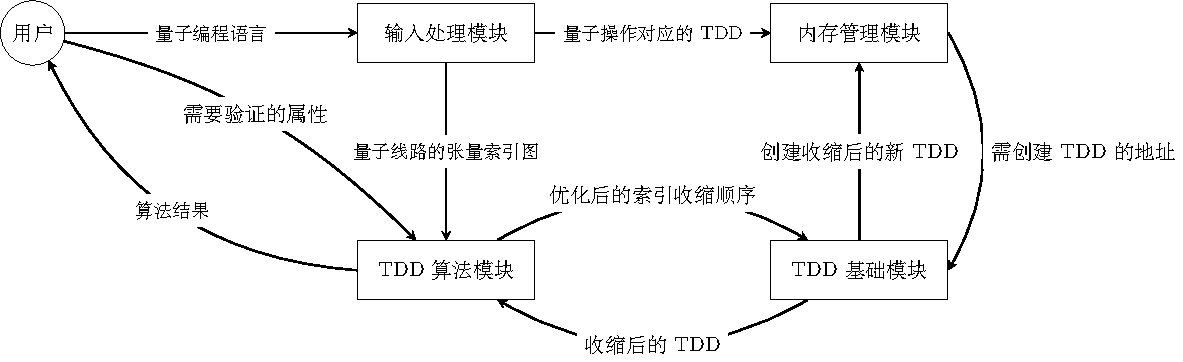
\includegraphics[width=\textwidth]{Img/alg_flow.pdf}
    \caption{软件模块之间的调用关系}
    \label{fig-flow}
\end{figure}
具体模块的作用如下:
\begin{itemize}
    \item \textbf{输入处理模块}:该模块的主要职责是处理输入数据,例如接收用OpenQASM\citep{cross2017open}格式编写的量子算法代码。其核心功能是将根据代码对应的量子操作,创建相应的TDD,并生成量子线路对应的张量索引图。鉴于当前存在多种量子编程语言,此模块的模块化处理能够显著提升系统的灵活性和兼容性。
    \item \textbf{TDD算法模块}:此模块为TDD提供更复杂的算法支持。例如,它能够调整节点收缩的顺序,以优化系统运行效率。该模块还可以导出TDD的树状结构图。树状结构图的导出功能则有助于用户更好地理解和分析TDD的结构。此外,它还能执行其他高级功能,如检验TDD是否存在于特定子空间中,对TDD进行分割。
    因此该模块的输入是量子线路的张量索引图,以及计算过程和计算结果的TDD。该模块的输出多种多样,可以是线路对应的TDD,也可能是某条属性是否满足。
    为了保留不同优化方案在不同量子线路的优点,目前在该模块中实现了\ref{sec-optimize}节中所有的优化方案。
    该模块是软件系统的核心,也是可拓展性最好的模块。
    \item \textbf{TDD基础模块}:该模块主要执行TDD之间的操作,例如TDD之间的收缩或加法。该模块的输入一般是张量收缩的顺序,输出是满足某些条件或者全部张量收缩后的TDD。
    \item \textbf{内存管理模块}:本模块负责管理TDD节点的存储和维护。每当需要创建新的TDD节点时,它会运用哈希算法与现有节点进行对比,以避免重复创建相同节点。因此该模块的输入主要是某个需要的TDD,输出则会返回该TDD的存储地址。该模块不仅减少了内存占用,还提高了软件系统的运行效率。

\end{itemize}

\begin{example}
    以例子\ref{ex-image-grover}中的Grover\_3量子线路的量子模型迁移系统为例。其对应的OpenQASM格式的量子编程代码如代码段1所示。
\begin{lstlisting}[language=Python, caption={Grover\_3量子线路的QASM代码}]
OPENQASM 2.0;
include "qelib1.inc";
qreg q[3];
ccx q[0],q[1],q[2];
h q[0];
h q[1];
x q[0];
x q[1];
h q[1];
cx q[0],q[1];
h q[1];
x q[0];
x q[1];
h q[0];
h q[1];
\end{lstlisting}
输入处理模块首先遍历量子线路,得到如图\ref{fig:addition}的量子索引图。然后根据每个量子门对应的矩阵形式和分配到的索引创建TDD。
之后输入处理模块将索引图输出给TDD算法模块。

TDD算法模块根据张量索引图和实际验证的属性,得到需要收缩的索引和对应的索引顺序。
在本例中,模型待验证的属性是\(\mathcal{T}_1(S)=S\)。其中子空间\(S\)的投影算子TDD结构如图\ref{fig:tdd_P}所示。\(\mathcal{T}_1\)为整个量子线路,因此需要收缩整个量子线路。按照图\ref{fig:addition}中的索引图对量子线路的收缩不进行优化,直接收缩后,得到TDD结构如图\ref{fig-tdd-grover}。将图\ref{fig-tdd-grover}和图\ref{fig:tdd_P}的两个TDD收缩后,得到的新的TDD就是子空间\(\mathcal{T}_1(S)\)投影算子的TDD表示。验证新的TDD表示是否在子空间\(S\)就可以验证属性。结果表明该量子迁移系统满足属性。

在本例的验证过程中,存在大量的优化空间。例如转移关系的TDD生成,即量子线路的收缩,可以通过量子线路拆分技术优化。子空间的TDD表示也可以通过子空间近似表示进行优化。如例\ref{ex-approx}中对\(S\)的空间表示进行了近似。而量子空间与转移的TDD都可以应用基于TDD结构的窗函数进行优化。如例\ref{ex-image-sub}中对\(S\)的TDD结构进行了窗函数的优化。
TDD算法模型中的优化方案是提升量子模型检测效率的关键。
\begin{figure}[htbp]
    \centering
    \includegraphics[height=10cm]{Img/reduced_tree.pdf}
    \caption{图\ref{fig:grover}中Grover\_3量子线路的TDD形式}
    \label{fig-tdd-grover}
\end{figure}
\end{example}
\section{本章小结}
本章主要介绍了在本文工作中采用的基于张量决策图(TDD)的量子模型检测方法。首先简单回顾了如何将量子系统建模为量子迁移系统。然后给出了计算子空间基、子空间并运算、以及系统一步迁移的算法。为加速模型检测,本章还介绍了一些针对性优化方法,包括索引顺序调整、addition线路拆分、contraction 线路拆分、基于TDD的划分,以及近似TDD表示等技术。最后,概述了软件系统的模块化设计,包括输入处理、内存管理、TDD基础运算和TDD算法等模块。

通过上述方法,本文以TDD为数据结构,构建了一种能高效计算量子模型检测中可达性分析问题的解决方案。TDD结合了BDD的紧凑表示和张量网络的计算优势,为解决量子计算中的模型检测问题提供了新的可能性。软件系统的模块化设计也为高效实现这一方案奠定了基础。总的来说,本章介绍的技术为量子模型检测提供了一种有前景的新方法。